\documentclass[
	ngerman,
	ruledheaders=section,%Ebene bis zu der die Überschriften mit Linien abgetrennt werden, vgl. DEMO-TUDaPub
	class=report,% Basisdokumentenklasse. Wählt die Korrespondierende KOMA-Script Klasse
	thesis={type=bachelor},% Dokumententyp Thesis, für Dissertationen siehe die Demo-Datei DEMO-TUDaPhd
	accentcolor=1b,% Auswahl der Akzentfarbe
	custommargins=true,% Ränder werden mithilfe von typearea automatisch berechnet
	marginpar=false,% Kopfzeile und Fußzeile erstrecken sich nicht über die Randnotizspalte
	%BCOR=5mm,%Bindekorrektur, falls notwendig
	parskip=half-,%Absatzkennzeichnung durch Abstand vgl. KOMA-Sript
	fontsize=11pt,%Basisschriftgröße laut Corporate Design ist mit 9pt häufig zu klein
%	logofile=example-image, %Falls die Logo Dateien nicht vorliegen
]{tudapub}


% Der folgende Block ist nur bei pdfTeX auf Versionen vor April 2018 notwendig
\usepackage{iftex}
\ifPDFTeX
\usepackage[utf8]{inputenc}%kompatibilität mit TeX Versionen vor April 2018
\fi

%%%%%%%%%%%%%%%%%%%
%Sprachanpassung & Verbesserte Trennregeln
%%%%%%%%%%%%%%%%%%%
\usepackage[english]{babel}
\usepackage[autostyle]{csquotes}% Anführungszeichen vereinfacht
\usepackage{microtype}


%%%%%%%%%%%%%%%%%%%
%Literaturverzeichnis
%%%%%%%%%%%%%%%%%%%
\usepackage[sorting=none]{biblatex}   % Literaturverzeichnis
\bibliography{Bibliography}



%%%%%%%%%%%%%%%%%%%
%Tabellen
%%%%%%%%%%%%%%%%%%%
%\usepackage{array}     % Basispaket für Tabellenkonfiguration, wird von den folgenden automatisch geladen
\usepackage{tabularx}   % Tabellen, die sich automatisch der Breite anpassen
%\usepackage{longtable} % Mehrseitige Tabellen
\usepackage{xltabular} % Mehrseitige Tabellen mit anpassarer Breite
\usepackage{booktabs}   % Verbesserte Möglichkeiten für Tabellenlayout über horizontale Linien
\usepackage{longtable}


\usepackage{paralist}
% left fixed width:
\newcolumntype{L}[1]{>{\raggedright\arraybackslash}p{#1}}
% center fixed width:
\newcolumntype{C}[1]{>{\centering\arraybackslash}p{#1}}
% flush right fixed width:
\newcolumntype{R}[1]{>{\raggedleft\arraybackslash}p{#1}}

\newenvironment{myitemize}
{ \begin{compactitem}
    \setlength{\itemsep}{0pt}
    \setlength{\parskip}{0pt}
    \setlength{\parsep}{0pt}
    }
{ \end{compactitem}                  } 

%%%%%%%%%%%%%%%%%%%
%Paketvorschläge Mathematik
%%%%%%%%%%%%%%%%%%%
%\usepackage{mathtools} % erweiterte Fassung von amsmath
%\usepackage{amssymb}   % erweiterter Zeichensatz
%\usepackage{siunitx}   % Einheiten


\usepackage{graphbox,graphicx}
\usepackage{float}
\usepackage{amsmath}




%Formatierungen für Beispiele in diesem Dokument. Im Allgemeinen nicht notwendig!
%\let\file\texttt
%\let\code\texttt

%\usepackage{pifont}% Zapf-Dingbats Symbole
%\newcommand*{\FeatureTrue}{\ding{52}}
%\newcommand*{\FeatureFalse}{\ding{56}}


\begin{document}

\Metadata{
	title=Reconstruction attacks on Federated Learning -- A comparison framework,
	author=Till Müßig
}

\title{Reconstruction attacks on Federated Learning}
\subtitle{A comparison framework}
\author[T. Müßig]{Till Müßig}%optionales Argument ist die Signatur, 
\reviewer{Prof. Dr. Max Mühlhäuser \and Aidmar Wainakh}%Gutachter

\department{inf}
\institute{Telekooperation}
%\group{Arbeitsgruppe}

\submissiondate{\today}
\examdate{\today}

%	\tuprints{urn=1234,printid=12345}
%	\dedication{Für alle, die \TeX{} nutzen.}

\maketitle
%\affidavit

\begin{abstract}
Conventional Machine Learning relies on a central server collecting huge datasets. Gathering other users' data naturally involves privacy issues. Federated Learning claims to solve these issues by shifting the learning process to the users' devices. In order to create a global training model, each participant calculates an update based on their own data and submits a fraction of it to a central server. With the personal data strictly remaining on the local device, privacy seems to be preserved \cite{kairouz2019advances}. However, recent studies show that contributing to the global model can leak private information. This leakage can be exploited to perform several attacks. One of these attacks is the reconstruction attack. It allows the reconstruction of the training data or class representatives from the global model or from the updates. Publications about this operate on various assumptions, preconditions and datasets. Yet it is difficult to compare them in the same context. In order to create a more general view on the topic, this thesis will implement a framework for federated learning on which various reconstruction attacks can be tested and compared to each other. The comparison framework will allow you to choose (about 3 different) attacks to run, as well as (about 3 different) datasets to be evaluated. The tool will be able to evaluate the attack performance and visualize it. Tuning Federated learning parameters and activating defense strategies will be an optional goal for this thesis. 
\end{abstract}

\tableofcontents

\chapter{Introduction}\label{sec:introduction}
Federated Learning is a novel technology that claims to enable Machine Learning among multiple datasets, while keeping each participant's data private from each other. Users train a local model on their local data and share parts of their model in order to create a global model that benefits each participant. Systems that currently run Deep Learning can be upgraded to Federated Learning and therefore allow a cooperation that would not be possible without it, due to privacy concerns. To give a better illustration of the concept one can imagine an application utilizing Federated Learning to allow facial recognition in CCTV. Panasonic published a white paper \cite{panasonic} and developed a system that recognises people, based on Deep Learning. Currently each operator has to maintain its own list of suspects (e.g. house banned people). With Federated learning a cooperation across all participators (e.g. a restaurant chain) would be possible without actually sharing images. Another example is health data, which might be shared between hospitals in order to allow cooperative learning. It might be tempting to upgrade learning tasks of many kinds into public federated learning networks in order to increase the available pool of samples. However, recent attacks, like those examined in Chapter \ref{sec:related_work}, showed that it is possible to recreate training data and class representatives, such as users faces, based on the models shared or the updates sent. In order to examine these threats more precisely and quantify the inherent privacy concerns, we will develop a framework, that simulates a Federated Learning Network and compares the suitability of different attacks for different settings. Before we get to the attacks and the framework, Chapter \ref{sec:background} provides helpful background knowledge on Deep Learning and Federated Learning.


\chapter{Background}\label{sec:background}
To provide a better understanding of the topic, this chapter provides helpful background knowledge of Deep Learning and its sub-field Federated Learning.

\section{Deep Learning}
Artificial Neural Networks (ANN or just NN) are a subcategory of Machine Learning Algorithms. They consist of multiple layers of interconnected computing units called neurons. Each neuron has a condition on which it will be activated. Its threshold is called weight. The first layer of input neurons could be a sensor input or a pixel in a picture. Output neurons can trigger actions like a classification of a picture as a cat. In order to show the desired behavior, a neural network adjusts its weights by training on examples \cite{schmidhuber2015deep}.\\
\\
As Sathya et Al.\cite{sathya2013comparison} state a NN can be classified on three levels. Based on its interconnection property (Feed Forward Networks vs. Recurrent Networks), regarding its application field (Classification, Association, Optimization or Self-organizing models) or depending on its data being either labeled or unlabeled and therefore supervised (SL) or unsupervised Learning (UL). The main characteristic of supervised learning is its training data being labeled with a ground truth property. SL algorithms learn the patterns that co-occur with this property and aim to predict it. In order to evaluate their success and adjust the weights accordingly, SL algorithms utilize loss functions, which quantify the difference between prediction and ground truth.\\
\\
One Supervised Learning Algorithm is called Gradient Descent (GD). Gradients describe how the outcome of a function varies when a parameter is changing. GD operates by calculating the gradients of the loss function, depending on the current weights. With other words, the algorithm calculates how the weights have to be adjusted in order to optimize prediction quality. By averaging the gradients over the training set, the resulting values hint the direction and the quantity in which weights should be shifted in order to reduce loss. The steps get smaller the closer the weights reach an optimum due to smaller gradient values near extrema. After some iterations the change rate falls below a threshold and the algorithm stops with a set of optimized weights. Calculating the gradients for each and every example is computational expensive. Therefore Stochastic Gradient Descent (SGD) simplifies the process by estimating the average gradient from a randomly picked subset of the training data called batch \cite{bottou2010large}. This algorithm takes an important role in Federated Learning. 


\section{Federated Learning}
Among a wide range of Deep Learning algorithms Stochastic Gradient Descent became an important factor for Federated Learning applications because it does not require the whole dataset at once. Instead it can work in parallel on different subsets of the data independently and sample batches from them. This can be utilized to bring the learning process from a central server to the users devices. With each participant solely working on its own data, Federated Learning drops the need of collecting data centrally. Meanwhile the benefits from evaluating a wide range of diverse users persist \cite{shokri2015privacy}.\\
\\
The term Federated Learning (FL) was coined by McMahan et Al. in \cite{mcmahan2016federated} and \cite{konevcny2016federated}. The authors presented a learning technique that allowed users to benefit from a shared model without urging them to share their own private data. Shokri and Shmatikov \cite{shokri2015privacy} described FL as privacy-preserving Deep Learning. McMahan's and Shokri's approaches have in common, that they utilize Stochastic Gradient Descent (SGD) in order to execute the learning process on different devices independently and in parallel.\\
\\
McMahan's version of FL uses Federated Averaging. A $C$-fraction of the $K$ clients calculates the gradients $g_k = \nabla F_k(w_t)$ for a $B$-sized batch of their dataset and their local model $w_t$. The server aggregates these gradients and performs an update $w_{t+1} \leftarrow w_t - \eta  \sum_{k=1}^K \frac{n_k}{n}g_k$. It uses a learning rate of $\eta$ and weights the sent in gradients with the amount of datapoints $n_k$ a client gathered divided by the total amount of datapoints $n$. 


\begin{figure}[H] 
  \centering
    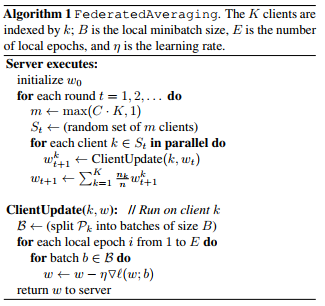
\includegraphics[width=0.6\textwidth]{Figures/FedAvg.PNG}
  \caption{FederatedAveraging by McMahan et Al. \cite{mcmahan2016federated}}
  \label{fig:fed_avg}
\end{figure}

In Shokri et Al.'s version of FL the clients will run Selective Stochastic Gradient Descent (SSGD). On client side the Protocol will approximate the optimal weights by iterating 4 steps:

\begin{enumerate}
    \item Download an update of the global model from the server
    \item Run SGD on a subset of the local data (batch) and update the local model
    \item Calculate the gradient vector that describes the change in the local parameters
    \item Upload a fraction of the gradients, picked either by random selection with threshold or by selecting the largest values
\end{enumerate}

Meanwhile the server updates the global model with the average of the sent in values.\\
\\
In order to protect privacy, the participants truncate the range of the uploaded gradients to $[-\gamma, \gamma]$ and add random noise that will eventually cancel out. Further only a $\theta _u$ sized fraction of the gradients will be uploaded and also only a $\theta _d$ sized fraction of the global model will be downloaded to minimize communication afford. The server takes measures to assure frequently updated values will get distributed more likely.\\
\\
McMahan et Al. denote four challenges for Federated Learning:\\
\begin{itemize}
    \item Non-IID: Each user's dataset is tailored to him or her and features different biases. It will not be a representation of the general distribution.
    \item Unbalanced: Some devices might provide a lot more training data than others.
    \item Massively distributed: The number of clients might be a lot larger then the average number of examples per client.
    \item Limited communication: Mobile devices might have a unreliant or expensive connection.
\end{itemize}{}
\\
Lyu et AL. \cite{lyu2020threats} denote three classes of FL.
\begin{itemize}
    \item Horizontal Federated Learning (HFL) operates on different participants, that collect similar properties from a wide range of users. Google's GBoard is one example for this.
    \item Vertical Federated Learning (VFL) refers to a network with large user overlaps among participators. However, each participator collects different properties from the user-base. A cooperation between an insurance, a finance company and a banking company might exemplify this.
    \item Federated Transfer Learning (FTL) includes scenarios with little user overlap and few common features. Therefore, it inherits challenges from both other classes
\end{itemize}
This thesis will focus on the standard scenario Horizontal Federated Learning. The challenges that the other scenarios bring would go beyond the scope of this thesis.\\
\\
Another differentiation can be made among centralized and decentralized parameter exchange. While the centralized approach gathers and distributes gradients via a central server, decentralized networks can exchange gradients directly to each other. The concept got visualized in Figure \ref{fig:centralized_decentralized} by Zhu et Al. \cite{zhu2019deep}.

\begin{figure}[H] 
  \centering
    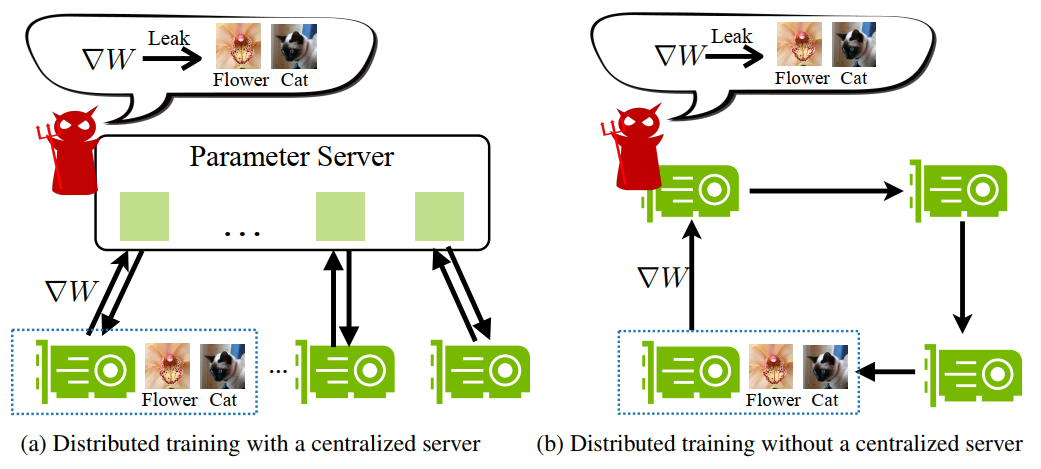
\includegraphics[width=1\textwidth]{Figures/centralized_decentralized.PNG}
  \caption{Centralized vs. Dezentralized parameter exchange by \cite{zhu2019deep}}
  \label{fig:centralized_decentralized}
\end{figure}

Regarding this differentation we will also stick to the standard scenario of centralized parameter exchange. 




\chapter{Related Work}\label{sec:related_work}
Related publications presented different kinds of attacks. Lyu et Al.\cite{lyu2020threats} distinguish them into two fundamental classes. Poisoning Attacks try to disturb the FL process in a way that will lead to misclassifications. Poisoning can either be targeted or random. Targeted Attacks aim for the misclassification of a certain sample, while random Attacks try to decrease overall accuracy. The second fundamental class, Inference Attacks, is characterised by the attempt to break the users privacy. It includes "Inferring Class Representatives", "Infering Membership" of certain samples in the training set, "Inferring Properties" of a users training set and "Inferring Training Inputs and Labels". Attacks that infer class representatives as well as training inputs are called Reconstruction Attacks. In this thesis we will focus on inferring class representatives.\\
\\
We acknowledge the critique McSherry\cite{mcsherry2017} published mentioning Shokri et Al.\cite{shokri2015privacy} and Hitaj et Al.\cite{hitaj2017deep}. He emphasised attacks on class representatives might or might not be a privacy break depending on the models architecture. For example the picture of a person averaged from a set of pictures from that individual labeled with his or her name is certainly privacy intrusive. In contrast an averaged picture generated from e.g. a female-male classifier might not reveal useful information about an individual if it does not generate the picture of an individual person, but an averaged representative of either class.





\section{Federated Learning under the GAN}
\subsection{Problem}
Hitaj et Al. \cite{hitaj2017deep} claim that federated learning is fundamentally broken. They showed that pictures of class representatives can be reconstructed from the global model by using a Generative Adversarial Network (GAN). The authors assume the attacker is participating in a Federated Network. His or her objective is to infer information about a particular class.

\subsection{Approach}
A GAN is a data generator that learns how to generate a sample with certain features. It utilizes some sort of discriminator, which decides whether a proper sample just has been created. Depending on this decision, the GAN will adjust its internal weights in order to get better results. In Hitaj et AL.'s Attack a GAN is used to create pictures similar to the originals. The global model is used as discriminator and therefore can not distinguish between originals and replicas anymore after some iterations. After training the GAN, the attacker will train his or her local FL model to misclassify these replicas as some arbitrary class c and submit his or her model. The global model gets tricked into classifiing samples from the targeted class as sample of the class c. This urges the victim, whos samples now get missclassified, to train its local model so it can distinquish again between the original picture and the GAN generated replica. The attacker can use the improved model, the victim uploaded, to further improve his or her GAN. After some iterations the attacker will end up with his or her GAN being able to reconstruct pictures looking just like the original.

\subsection{Result}
The authors benchmarked their GAN versus a Model Inversion (MI) approach. The main difference here is that the MI operates on the model after it has been trained, while the GAN influences the training process as described previously. Their first experiment was to classify and reconstruct the digits from the MNIST dataset. The  result is shown in Figure \ref{fig:mi_vs_gan}.

\begin{figure}[H] 
  \centering
    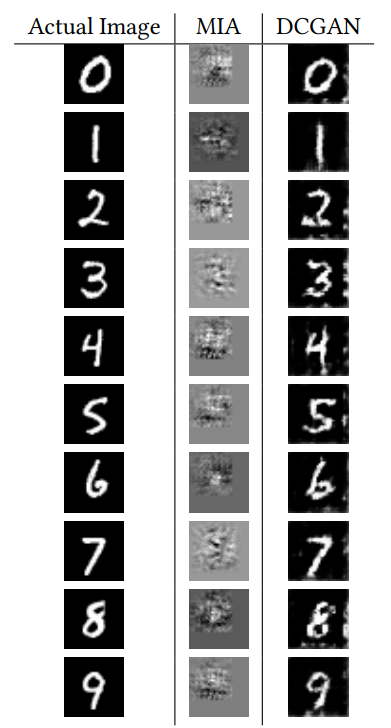
\includegraphics[width=0.4\textwidth]{Figures/MI_vs_GAN.PNG}
  \caption{Model Inversion vs. Generative Adversarial Network  by Hitaj et Al. \cite{hitaj2017deep}}
  \label{fig:mi_vs_gan}
\end{figure}

Their second experiment was based on the AT\&T face dataset. They showed that the defence strategy random obfuscation of the gradients does not prevent their attack, even though it may guarantee differential privacy for the inputs. The parameter $\frac{\epsilon}{c}$ is the privacy budget and manages how often a gradient can be published. A comparison can be seen in Figure \ref{fig:gan_face}


\begin{figure}[H] 
  \centering
    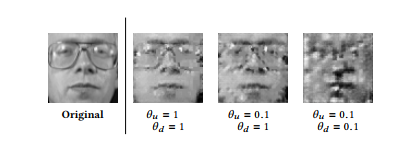
\includegraphics[width=0.6\textwidth]{Figures/face_no_dp.PNG}\\
    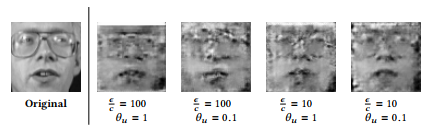
\includegraphics[width=0.6\textwidth]{Figures/face_dp.PNG}
  \caption{ Generative Adversarial Network reconstructing faces without (upper figure) and with differential privacy enabled (lower figure), different rates of privacy budget $\frac{\epsilon}{c}$ and various upload and download fractions per iteration by Hitaj et Al. \cite{hitaj2017deep}}
  \label{fig:gan_face}
\end{figure}

\subsection{Connection}
This approach creates promising results. However, it is open how this approach will adapt to other conditions, where samples of the same class might differ more or defensive measures were taken. It might be interesting to implement it, study this question and compare it to other approaches.





\section{Model Inversion Attacks that Exploit Confidence Information and Basic Countermeasures}
\subsection{Problem}
Fredrikson et Al. \cite{fredrikson2015model} developed their approach to be used with Machine-Learning-as-a-service platforms like Microsoft Machine Learning, Google's Prediction API or BigML. These platforms require uploading a training set and provide an API that answers classification tasks. Some of these platforms allow selling the models and/or provide access to the classification function to other users, charging them per prediction query. Selling the model is called a white-box setting, while providing classification query access, without revealing the model, is called a black-box setting. Models trained by Federated Learning are necessarily shared with each participant. Therefore, FL could be interpreted as a white-box scenario. In this case it might be possible to transfer the Machine-Learning-as-a-service attack onto Federated Learning. In Fredrikson et Al.'s study, they were able to recreate faces out of a facial recognition API.
 
 \subsection{approach}
 A common Model Inversion approach starts with an incomplete input vector and completes the missing part. It iterates over every possible combination and calculates the probability of the vector being classified correctly. Nominal-Valued features can be estimated with this method, but it fails when it tries to infer real-valued features, due to the huge combination space. Fredrikson et Al.'s approach overcomes this problem by utilizing confidence information (CI). CI is generated during the model training and evaluates the probability of an example being correctly classified. The authors MI attack starts with a random image and calculates the probability of every pixel to be part of a picture in the targeted class. Using Gradient Descent the probabilities can be optimized until the loss function falls bellow a threshold.
 
 \subsection{Result}
 Even though the reconstructed Images were slightly blurred, they were still recognizable. Some of the tested participants could match the reconstructed pictures to the right person with 95\% accuracy.

\subsection{Connection}
This study does require side information for its prediction, namely the confidence score. It should be possible to implement this into a Federated Learning network and see if it provides an advantage over the other attacks.







\section{Updates-Leak: Data Set Inference and Reconstruction Attacks in Online Learning}
\subsection{Problem}
The reconstruction attack developed by Salem et Al. \cite{salem2019updates} shows another attack vector. They assume an attacker to aquire two different versions of a model. The difference from one set to another hints the data that has been used for this update. Using a GAN the authors create training data that might have caused this model change. 

\subsection{Approach}
This attack is an encoder-decoder styled approach. The encoder trains on two models, one before and one after an update. It learns what an update, that archived the observed change in sample classification, probably looked like. This attack might be performed by the server or a man-in-the-middle, that knows the prior and the posterior model of a client. They developed four different attacks that differ in the update size (single or multi-sample) and in the inference goal (labels or reconstruction) as follows:
\begin{enumerate}
    \item Single-Sample Label Inference Attack: Predict used label in update
    \item Single-Sample Reconstruction Attack: Recreate updating sample
    \item Multi-Sample Label Distribution Estimation Attack: Predict label distribution in update
    \item Multi-Sample Reconstruction Attack: Recreate all updating samples
\end{enumerate}

Despite inferring the labels of an update is interesting as well, we focus on the reconstruction attacks. Especially the Multi-Sample Reconstruction Attack suits our needs. This attack takes the vector from the encoder and feeds it into the Conditional Best of Many Generative Adversarial Network (CBM-GAN). The constructed samples get clustered and shrinked to one representative image for each cluster. 

\subsection{Results}
This attack was benchmarked using the CIFAR-10 dataset. The authors took a snapshot of the classification model before and after an update of 100 pictures and fed it into their approach. Figure \ref{fig:cbm_gan} shows the targeted picture along with the best examples the GAN created. The pictures are blurry but hint the original picture.

\begin{figure}[H] 
  \centering
    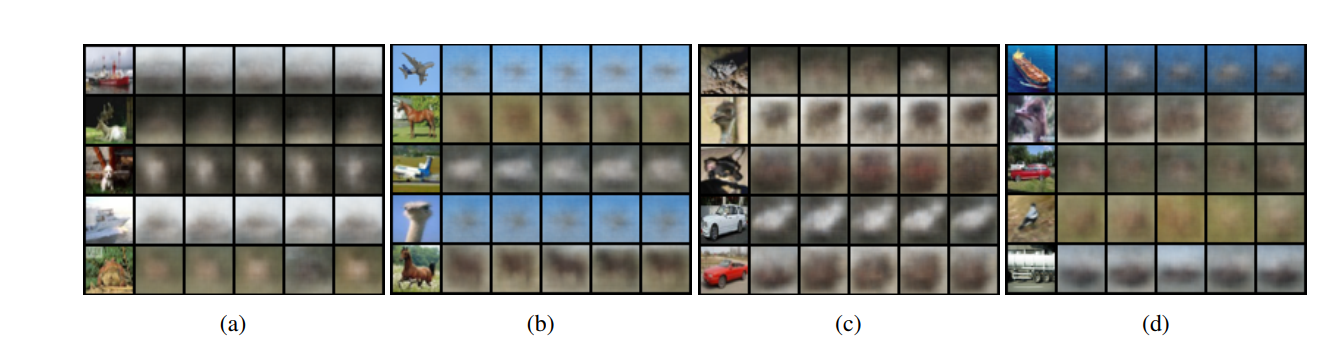
\includegraphics[width=1\textwidth]{Figures/cbm_gan.PNG}
  \caption{ CBM-GAN reconstructed images from the CIFAR-10 dataset by Salem et Al. \cite{salem2019updates}.}
  \label{fig:cbm_gan}
\end{figure}


\subsection{Connection}
This attack is special as it needs two models and creates multiple pictures at once. The images from this paper look more blurred than in other approaches. The results of this framework will show if this difference still remains under more similar conditions or if the authors just chose a harder scenario than the others.







\section{(Improved) Deep Leakage from Gradients}
\subsection{Problem}
Reconstruction Attacks like the GAN approach tried to synthesize pictures with a fixed label, that caused a participant to send out a certain gradient update. The Deep Leakage from Gradient (DLG) approach \cite{zhu2019deep} takes a twist on this and alters the input picture as well as the output label in order adjust the attacker's gradient to match the victim's gradient.

\subsection{Approach}
The Deep Leakage from Gradients approach begins with a random generated input picture and output label. The victim calculates its prediction from its picture, calculates the loss and its gradients and sends out the gradient update. The attacker, who intercepted the update, calculates the same steps with his or her dummy data. After that, he or she calculates the optimal input and output values, which minimize the squared vector distance between the original and the dummy gradients. With the updated dummy input and output, the process starts over until the gradient's distance falls below a threshold or the process is stopped. The algorithm and its structural visualization can be seen in Figure \ref{fig:dlg}.

\begin{figure}[H] 
  \centering
    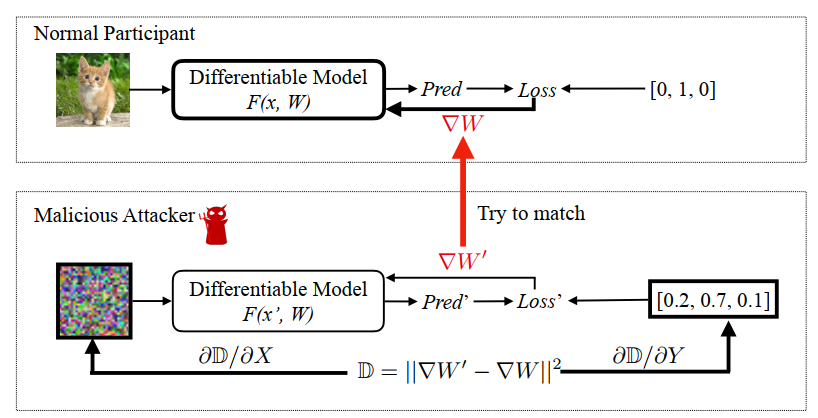
\includegraphics[width=0.9\textwidth]{Figures/DLG_structure.PNG}\\
    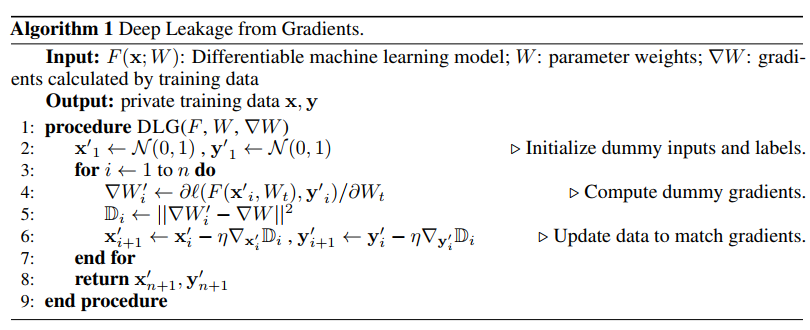
\includegraphics[width=0.9\textwidth]{Figures/DLG.PNG}
  \caption{Deep Leakage from Gradients by \cite{zhu2019deep}}
  \label{fig:dlg}
\end{figure}



\subsection{Result}
Figure \ref{fig:dlg_result} shows some examples of recreations after a given amount of iterations. Starting with the random dummy values the pictures reach almost perfect results after 500 iterations, apart from a few pixel fragments. The result of Melis et Al.'s \cite{melis2019exploiting} recreation is shown as comparison.

\begin{figure}[H] 
  \centering
    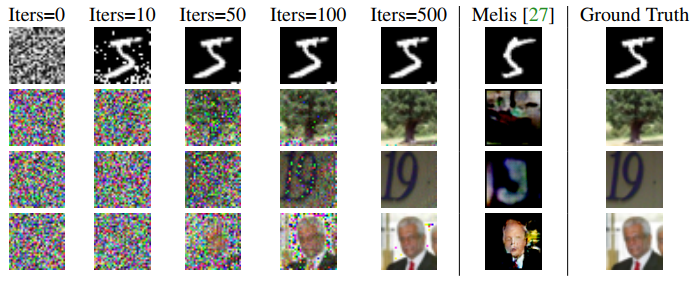
\includegraphics[width=0.9\textwidth]{Figures/DLG_result.PNG}\\
  \caption{Reconstructed images with Deep Leakage from Gradients by \cite{zhu2019deep}}
  \label{fig:dlg_result}
\end{figure}

\subsection{Improved Deep Leakage from Gradients}
Zhao et Al. \cite{zhao2020idlg} published their approach building directly on DLG. The authors improved the reconstruction by adding a interim stage. In this stage, they use the fact that the gradient of the classification loss of correct labels in the output layer and the last layer weights lie in the interval [-1, 0], while they lie in [0,1] for other labels. With this rule it is possible to extract the ground-truth labels from an update with 100\% accuracy. This facilitates better data extraction. The next steps are according to regular DLG the generation of a random dummy input, the calculation of the dummy gradients and the Gradient Descent optimisation of Gradient difference. Zhao et Al. compared their algorithm with regular DLG for the three datasets MNIS, CIFAR-100 and LFW. While DLG found the ground-truth labels in between 79\% and 89\% of the cases iDLG succeded with 100\% accuracy. The image reconstruction also profited from the improvement. Figure \ref{fig:dlg_vs_idlg} shows the percentage of good reconstructed images with a certain threshold, that determains how accurate a picture has to be for this. They used the mean square error to evaluate deviation.

\begin{figure}[H] 
  \centering
    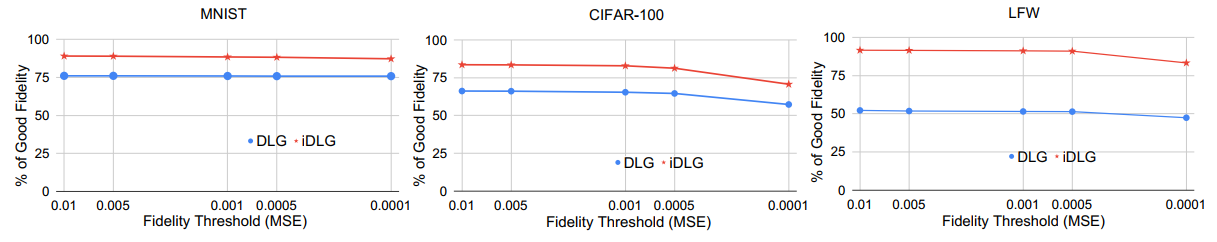
\includegraphics[width=1\textwidth]{Figures/DLG_vs_iDLG.PNG}\\
  \caption{Comparisson between iDLG (Zhao et Al.) and DLG (Zhu et Al.).\cite{zhao2020idlg}}
  \label{fig:dlg_vs_idlg}
\end{figure}


\subsection{Connection}
Both attacks show promising results and it would be interesting to add them to this framework in order to compare them to other approaches.





\chapter{Research Problem}\label{sec:research_problem}
Federated Learning is a novel technology. Its main feature is the claimed privacy gain. However, this new technology comes with new attack vectors. Recent research showed privacy is at risk. Each paper describes a certain setting under which the attack is evaluated. To our knowledge currently there has not been a framework yet, that features multiple attacks in the same setting. The main goal of this thesis is the comparison of several reconstruction attacks. We will try to create a unified setting and equal preconditions. Also fair metrics have to be elaborated to make the approaches comparable. The framework should be able to create a visual comparison to illustrate the accuracy of the different attacks. Further it should enable the user to adjust preconditions. He or she could tune the settings, choose attacks to run, choose a dataset and adjust network parameters.\\
\\
One optional goal could be the implementation of defensive strategies. Recent papers suggested measures that claim to defend against reconstruction attacks. A comparison on how useful these are with different attacks would be interesting.\\
\\
A second optional goal might be the combination of different attacks in order to increase their accuracy. Some of the current approaches create noisy images and have limited possibilities. Combining different attack vectors might create synergy and improve the results.






\chapter{Methodology}\label{sec:methodology}
In order to make the studied attacks comparable, we will develop and implement a framework that simulates a Federated Learning Network. The FL models's task will be simple image classification. On top of that, the attacks will try to recreate class representatives. The main challenge of this thesis is the development of a suitable architecture for this framework that allows performing the different attacks and adjusting the conditions. The second challenge will be to find a way to compare the created images. As an optional challenge, defense strategies and additional combined attacks might be implemented if the previous steps take less time then expected.







\chapter{Evaluation}\label{sec:evaluation}
One of the objectives is to quantify the success of different attack vectors and find a way to compare them. The framework should enable the user to study the impact different settings will have on different attacks. Datasets and settings should be adjustable.




\section{Datasets}
In order to analyse the attacks and make them comparable with others, we will test them with datasets frequently used in Deep Learning related papers (e.g. \cite{shokri2015privacy}, \cite{zhu2019deep}). Currently we consider the following datasets:
\begin{enumerate}
    \item MNIST: Dataset consisting of 60.000 training and 10.000 test examples of hand written black and white digits.
    \item SVHN: Dataset consisting of 600.000 training and 10.000 test examples of house numbers taken from Google Street View
    \item CIFAR-10: Dataset consisting of 50.000 training and 10.000 test examples for each of ten classes (airplane, automobile, bird, cat, deer, dog, frog, horse, ship and truck)
    \item AT\&T Database of Faces: Dataset with 10 different portrait pictures for each of 40 different individuals.
\end{enumerate}




\section{Settings}
The framework should enable the user to adjust settings like the size of the Federated Learning Network, the used dataset, the distribution of the samples, learning rates, iterations or defensive strategies. The exact adjustable options will be determined in a later stage of this thesis.



\section{Metric}
The metric used will also be determined in a later phase of this thesis. The introduced studies already proposed ways to measure the accuracy of the attacks in different ways. We will try to choose one or two and adapt them, so we can compare the approaches. The suggested metrics include MeanSquareError (MSE) of the generated pictures. Another metric suggests to let human test subjects match the replicas to the originals and evaluate the result. This framework wants to let the user try out different settings with an automatic feedback. Therefore human evaluation based on visual comparison doesn't suit its needs. However, a visual lineup of the best results for different attacks might be interesting to generate visuals for this thesis.




\printbibliography

\begin{appendix}
 \chapter{Timetable}
 \small
%\hskip-1.5cm
\begin{longtable}[H]{ | L{13cm} | l |} 
\hline
 Milestones & due \\ \hline
 
 Phase 0: Exposé 
 \begin{myitemize}
     \item Research the background of Deep Learning and Federated Learning
     \item Research on different attacks on Federated Learning
     \item Write a first draft for "Introduction", "Background", "Related Work", "research problem" and "methodology"
     \item Register the thesis.
 \end{myitemize}  
 & 15.05.20   \\ \hline
 
 Phase 1: Concept
 \begin{myitemize}
     \item Continue to write "research problem" to a "75\% finished" state
     \item Define the architecture
     \item Define the attacks in "Related Work" to a "75\% finished" state
     \item Define the datasets and metrics in "Evaluation" to a "75\% finished" state
     \item Continue to write "methodology" to a "50\% finished" state
 \end{myitemize}  
 & 01.06.20   \\  \hline
 
 Phase 2: Implement 
 \begin{myitemize}
     \item Prepare the datasets
     \item Implement the FL network and make sure it works as intended
     \item Implement the attacks and make sure they work as intended
     \item Make the settings adjustable and make sure they do not break the framework
     \item Implement a visualisation for the results
     \item Meanwhile continue to write "methodology" to a "75\% finished" state
 \end{myitemize}  
 & 01.08.20   \\  \hline
 
 Phase 3: Measure  
 \begin{myitemize}
     \item Run the attacks and gather the findings
     \item Try different settings, tweak configurations
     \item Find a way to present the findings in the paper
     \item Write "evaluation" to a "75\% finished" state
 \end{myitemize}  
 & 01.09.20  \\  \hline
 
 Phase 4: Finish  
 \begin{myitemize}
     \item Finish to write all chapters
 \end{myitemize}  
 & 01.10.20   \\  \hline
 
 Phase 5: Pre-Submission  
 \begin{myitemize}
     \item Prepare the presentation
     \item Check citations, spelling, packet usage, structure and logic of the thesis paper
     \item Code-style and documentation 
 \end{myitemize}  
 & 15.10.20   \\  \hline
 
 Phase 6: Presentation  
 \begin{myitemize}
     \item Hold the presentation
     \item Maybe include feedback into the final submission
     \item Finish before the next semester starts on 01.11.20
 \end{myitemize}  
 & 31.10.20  \\  \hline

\end{longtable}



\end{appendix}
	
\end{document}
